\chapter{Modular and Efficient Flock Pattern Identification}
\label{chp:solution}
\section{Generic System Architecture}
\label{sec:architecture}
After the related work research that was performed, we noticed a lack of system architecture in order to solve data
spatio-temporal pattern detection problems. So far, no previous work has provided an system architecture that could be
easily extensible and reusable for helping to address the myriad of issues related to spatio-temporal pattern detection.

We first tried to approach this problem in a more generic fashion, since all moving pattern mining problem has the same
workflow:

\begin{enumerate}
    \item Connect to a spatio-temporal data source
    \item Retrieve and aggregate spatio-temporal data
    \item Process and mine that data in order to find the desired pattern or extract the desired information
\end{enumerate}

With that in mind, we designed a modular and easily extensible architecture that can fit for almost all spatio-temporal
data mining problem, which is depicted by \figref{fig:architecture}. One can notice that we focus on 4 key building
blocks, that can be easily registered/unregistered according to the targeting problem: (1) \acp{dsc}; (2) \acp{dd}; (3)
\acp{dl} (Data aggregators); (4) \acp{dp}.

In layer (1) we are concerned on how to retrieve the data, meaning how to communicate properly to the data source in
order to be able to extract each record of spatio-temporal from it. Thus, each \ac{dsc} depicted in the \textit{Data
Connectors' Module} in \figref{fig:architecture} represents a logical piece that knows how to connect to and extract
data from a specific data source. We can have a \ac{dsc} that knows how to connect to a MySQL database, or another one
that can connect to a cloud based storage system like \ac{aws} DynamoDB, or even a \ac{dsc} that simply connects to an
online data stream and listen for incoming data.

\begin{figure}[h!]
    \centering
    \caption{Generic System Architecture overview}
    \centerline{\includegraphics[width=\linewidth]{images/architecture.png}}
    \footnotesize{Source: Made by the author.}
    \label{fig:architecture}
\end{figure}

After connecting and retrieving data from a data source, we need to clean, decode and translate the incoming raw data to
a format that is simple and understandable to our system. Aiming at achieving that, we will have a \ac{dd} component,
which knows how to interpret the raw data format that comes from a \ac{dsc} and translate it to a format that layer (3)
can understand. We can see in \figref{fig:architecture} that a \ac{dd} can register itself to a \ac{dsc} in order to
receive each data record that such \ac{dsc} gathers from a data source. It is important to note that a \ac{dd} can
register to only one \ac{dsc}, but a \ac{dsc} can have multiple \acp{dd} registered to it.

In any problem of data mining, aggregation is one of the most important phases, since it is there that the data
gathering happens and necessary arrangements are made in order to get the data ready for processing. In our system that
is represented by layer (4), which we call the Data Listeners' Module. We can have multiple types of \acp{dl} in that
module, and each of them can perform different types of aggregation and pre-processing depending on the final goal.  For
example, we could have an aggregator (or listener) that \textit{bucketize} the \ac{gps} points by their timestamp and
filter out outliers, before sending to processing, or another one that performs point interpolation in order to reduce
trajectory uncertainty. Similarly to the \ac{dd} module, a \ac{dl} can only register itself to one \ac{dd}, but a
\ac{dd} can have multiple \acp{dl} registered to it. Later on we will see a \ac{dl} implementation as one of the
contributions of this dissertation, which will perform a \textit{bufferized} aggregation of points.

The last, but not least, remaining piece is the Data Processors' Module, in layer (5). It is there that we will have the
intelligence to perform a data mining task that will generate insights for decision making, detect moving patterns and
the forth. We can have a \ac{dp} that detects flock patterns, another one that detects convergence patterns and even
another \ac{dp} that provides traffic information in real time, to name a few. Following the pattern of the
aforementioned modules, each \ac{dp} can only register itself to a single \ac{dl}, but a \ac{dl} can have multiple
\acp{dp} registered to it. This dissertation will present a novel \ac{dp} for detecting flock patterns, based on the
\ac{bfe} algorithm proposed by Vieira et al. \citep{vieira}.

Researchers and data analysts can leverage from the proposed architecture in order to tackle multiple problems at once,
reusing components that can serve other spatio-temporal pattern mining problems.

\section{Aggregation and data processing efficiency}
\label{sec:aggreg_efficiency}
By analyzing some of the algorithms proposed in \secref{sec:rel_flocks} and their respective running times, we noticed
that most of the \ac{cpu} cycles were spent in analyzing disks that will not generate flock patterns, due to the points
not being present in $\delta$ consecutive time slots. In all algorithms, disks generated in time slot $t_{i+1}$ are
compared with those generated in $t_{i}$ in order to check if an extension to a potential flock pattern is found. This
operation has $O(nm)$ complexity, with $n$ being the number of disks and $m$ the number of potential flocks from
previous time slots.  Additionally, for each comparison between a disk and a potential flock, an intersection operation
between them needs to be made.

Things get even worse in algorithms like \ac{bfe}, where a new created disk $d_j$ is checked if it is either subset or a
duplicate of a previously found disk $d_i$ (as already mentioned in \secref{subsec:disk_discovery}). The running time of
this step can result in a $O(n^2)$ time complexity in the worst case (with $n$ being the number of disks generated by
that time slot) requiring an intersection operation between each pair of disks that are being compared. We can reduce
significantly that number of disks by only creating disks with points that can potentially form a flock pattern, i.e.
with points that appears in the dataset for $\delta$ consecutive time slots. In order to show how expensive those disk
operations can be, we measured the time spent in them using the datasets that we will use in our experiments and show
the results in \figref{fig:time_consumption}. The analysis shows that the disk and flock related operations can reach
99\% of the overall processing time of the algorithm.

\begin{figure}[h!]
    \centering
    \caption{Percentage of time spent between disk and flock processing tasks against other tasks in the algorithm}
    \centerline{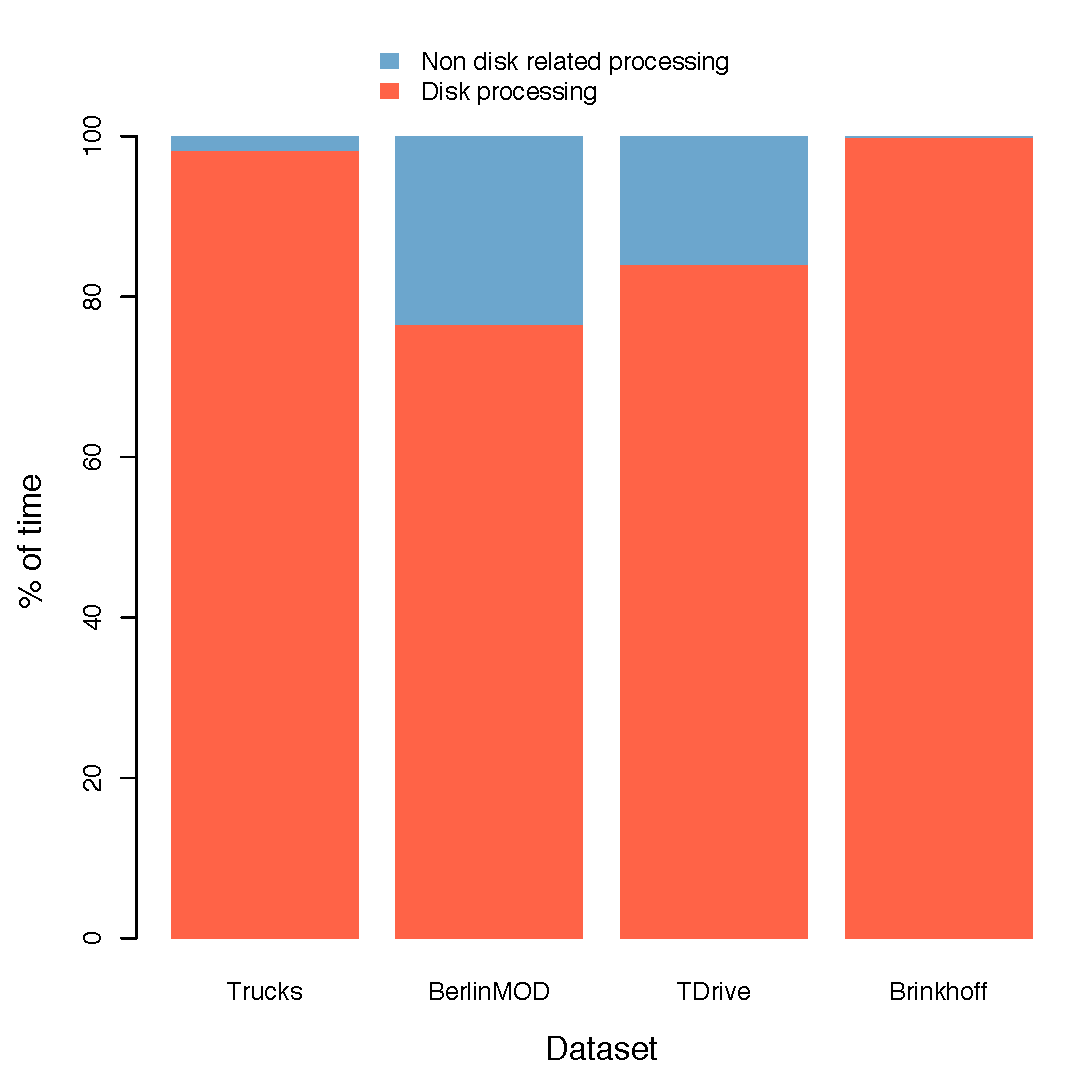
\includegraphics[width=0.7\linewidth]{images/timeConsumption.eps}}
    \footnotesize{Source: Made by the author.}
    \label{fig:time_consumption}
\end{figure}

\begin{figure}[h!]
    \centering
    \caption{Sequence of disks in 4 consecutive time slots and the points that were clustered to them}
    \centerline{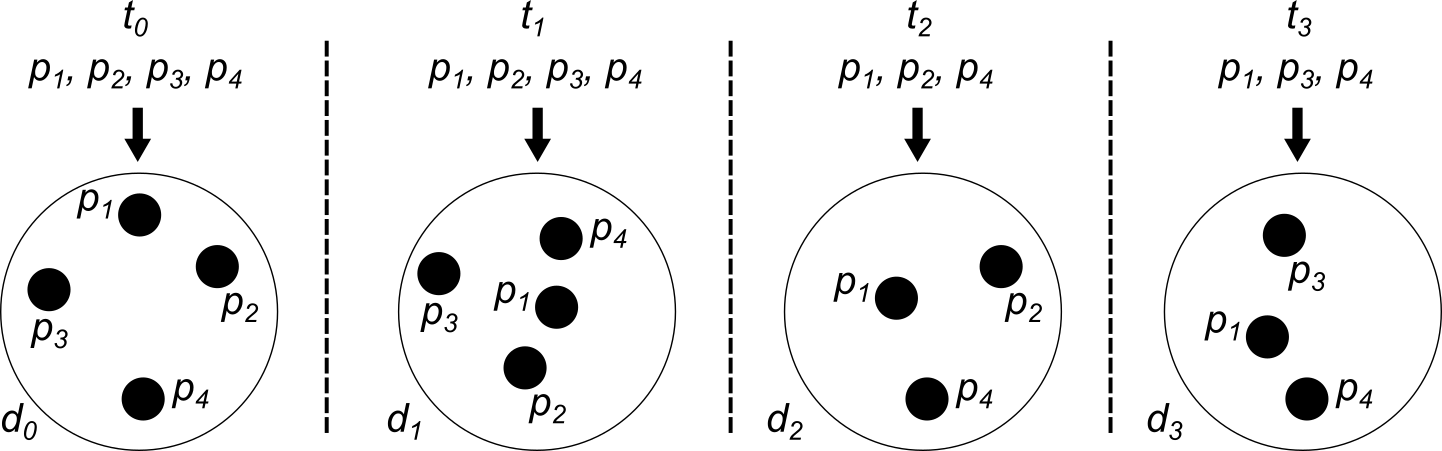
\includegraphics[width=\linewidth]{images/disks_2.png}}
    \footnotesize{Source: Made by the author.}
    \label{fig:disks}
\end{figure}

Consider the \ac{bfe} algorithm running example depicted in \figref{fig:disks}, where we are looking for flock patterns
having $\mu=4$ and $\delta=4$ as parameter values. As we can see, in time slot $t_0$ our dataset reported points
$p_1,p_2,p_3$ and $p_4$ and, due to the proximity between them, disk $d_0$ was created enclosing all four points.  In
the subsequent time slot $t_1$ the same points were reported and again the \ac{bfe} algorithm was able to create another
disk $d_1$. However, in time slot $t_2$, $p_3$ was not present and the disk $d_2$ only contained three points, which is
not enough to represent a flock pattern because of the number of trajectories being less than $\mu = 4$. With the disk
$d_2$ being invalid in $t_2$, we will need to discard disks $d_0$ and $d_1$ created in the previous time slots, since
they cannot generate a flock pattern starting from $t_0$. Hence, we could avoid the creation of disks $d_0$ and $d_1$ if
we would know in advance that $p_3$ was missing in $t_2$, saving \ac{cpu} cycles of disk comparisons in $t_0$ and $t_1$.
We argue that when scaled to a dataset of millions of records, doing real-time analyses, such processing for checking
disks subsets and flock extension, performed by regular algorithms (like \ac{bfe}), will lead to severe degradation in
performance. With that in mind, we can say with high confidence that reducing the processing time spent with unnecessary
disks that will not generate flock patterns, can dramatically reduce the overall processing time of a flock detection
algorithm.

\section{BitDF}
\label{sec:bitdf}

Our solution consists on using \textbf{Bit}maps for \textbf{D}isk \textbf{F}iltering (\acsu{bitdf}\label{acro:bitdf}),
based on the \ac{bfe} algorithm. \ac{bitdf} is basically a Data Listener and a Data Processor component, as those in the
architecture presented in \secref{sec:architecture}. We call them \ac{gsb} and \ac{fp} the \ac{dl} and \ac{dp}
respectively, and will have each of them keep track of the history of every $O_{id}$ in time.

\begin{algorithm}[h!]
\caption{\ac{gps} Stream Buffering}
\label{alg:gpsb}
\begin{algorithmic}[1]
    \State $pointBuffer \gets map\{index, \{id, point[...]\}\}$
    \State $presenceMap \gets map\{id, bitmap\}$
    \State $lastTimeslot \gets -1$
    \State
    \Procedure{AddPointPresence}{$id$}
        \State $mask \gets \Call{ShiftLeft}{1, pointBuffer.size - 1}$
        \State $presence \gets \Call{BitOr}{presenceMap[id], mask}$
        \State $presenceMap[id] \gets presence$
    \EndProcedure
    \State
    \Procedure{ShiftPresenceMaps}{}
        \ForAll {$id \in \Call{Keys}{presenceMap}$}
            \State $shifted \gets \Call{ShiftRight}{presenceMap[id], 1}$
            \State $presenceMap[id] \gets shifted$
        \EndFor
    \EndProcedure
    \State
    \Procedure{ReceivePoints}{}
        \Loop
            \State $point \gets gpsPointStream.dequeue$
            \State $timeSlot \gets point.timestamp / timeSlotSize$
            \If{$timeSlot > lastTimeslot$}
                \If{$pointBuffer.size \ge \delta$}
                    \State \Call{Fp.Process}{pointBuffer.first}
                    \State \textbf{delete} $pointBuffer.first$
                    \State \Call{ShiftPresenceMaps}{}
                \EndIf
                \State $lastTimeslot \gets timeSlot$
            \EndIf
            \State $pointBuffer[timeSlot][point.id].append(point)$
            \State \Call{AddPointPresence}{$point.id$}
        \EndLoop
    \EndProcedure
\end{algorithmic}
\end{algorithm}

Algorithm~\ref{alg:gpsb} shows a big picture of how \ac{gsb} will work once it receives spatio-temporal data records
from a \ac{dd}. It will listen to the incoming \ac{gps} point stream in the procedure \textsc{ReceivePoints}, add each
point to the \textit{pointBuffer} structure (which is a hash map of points by time slot) and record the presence in time
of that $O_{id}$ in its bitmap structure by calling \textsc{AddPointPresence}. When \ac{gsb} has buffered $\delta$ time
slots (line 23) it will then send the points of $timeSlot - \delta$ to \ac{fp}. After \ac{fp} is done with processing
the points, \ac{gsb} will discard the presence maps of $timeSlot - \delta$ (which corresponds to the points sent to
\ac{fp}), by calling \textsc{ShiftPresenceMaps}, and also discard the points collected in $timeSlot - \delta$, which
were already processed by \ac{fp}. The flow continues indefinitely by buffering the points from the next time slot $t_i$
and send the points from $t_{i - \delta}$ to \ac{fp} for processing. It is worth noting that \textit{timeSlotSize},
referred in line 21, represents the time slot $\sigma$ introduced in \secref{sec:tech_data}.

Using \figref{fig:disks} as an example, we can see in \tabref{tab:bitmaps} the state of the \ac{gsb} bitmaps for each
$O_{id}$ after receiving the points in $t_3$. With those bitmaps, we can easily look up for a specific point occurrence
in time and check whether that point in that specific time slot can potentially form a flock pattern or not. We do that
by checking if that $O_{id}$ appears for $\delta$ consecutive time slots in the dataset, i.e. it has $\delta$
consecutive bits set to 1. The bitmaps in \ac{gsb} will always refer to the "future" of a specific $O_{id}$.

\begin{table}[h!]
    \renewcommand{\arraystretch}{1.3}
    \caption{Bitmaps in \ac{gsb} after buffering four time slots}
    \label{tab:bitmaps}
    \centering
    \begin{tabular}{c | c}
        \toprule
        $O_{id}$ &   Bitmap\\
        \toprule
        1        &   1111\\
        \bottomrule
        2        &   0111\\
        \bottomrule
        3        &   1011\\
        \bottomrule
        4        &   1111\\
        \bottomrule
    \end{tabular}
\end{table}

Our \ac{dp} is explained in more detail by Algorithms~\ref{alg:fp_helpers} and~\ref{alg:fp} as follows. In
Algorithm~\ref{alg:fp_helpers} we start by first listing the procedures that will help the core procedure of \ac{fp}
(the \textsc{Process} procedure, in Algorithm~\ref{alg:fp}). It is also in Algorithm~\ref{alg:fp_helpers} that we list
the most important piece of this \ac{dp} that allows us to achieve such good optimizations, in both \ac{cpu} cycles and
number of disks generated, which is the \textsc{IsPointEligible} procedure. Such procedure is responsible to put
together what happened in the \textit{past} and what is going to happen in the \textit{future} for a given point $p$, in
order to decide whether $p$ can be part of a potential flock pattern or not. It does that by concatenating, for a given
$O_{id}$, the bitmap from \ac{fp} with the bitmap from \ac{gsb} (line 5 of Algorithm~\ref{alg:fp_helpers}) and searching
for a sequence of $\delta$ bits set to 1 (lines 6 to 15 of Algorithm~\ref{alg:fp_helpers}). That search is performed by
combining AND and XOR bitwise operations against the presence bitmap assembled in line 5 of
Algorithm~\ref{alg:fp_helpers}. If a sequence of $\delta$ bits set to 1 is found, we can state with confidence that such
point $p$ can potentially be part of a flock pattern. Later on, if a potential flock is found in a time slot $t_i$ and
$p$ is part of it, we need to update the \ac{fp}'s bitmap of that point so when we process points of time slot $t_{i+1}$
we have the correct bitmap representation of $p$ and that is where \textsc{MapPointFlock} (line 20) comes to play.
\textsc{MapPointFlock} does that by prepending 1 to $p$'s bitmap in \ac{fp} module by performing an OR bitwise
operation.

\begin{algorithm}[h!]
\caption{Flock Processor Helper Procedures}
\label{alg:fp_helpers}
\begin{algorithmic}[1]
    \State $buffered \gets 0$ \Comment max time span of the current flocks, max value is $\delta$
    \State $flockMap \gets map\{id, bitmap\}$
    \State
    \Procedure{IsPointEligible}{$id$}
        \State $presence \gets \Call{Concat}{presenceMap[id], flockMap[id]}$
        \State $eligibleMask \gets \Call{ShiftLeft}{1, \delta} - 1$
        \State $range \gets pointBuffer.size + buffered$
        \State $checks \gets \Call{Max}{1, range - \delta + 1}$
        \While{$checks > 0$}
            \State $tmp \gets \Call{BitAnd}{presence, eligibleMask}$
            \If{\Call{BitXor}{$tmp, eligibleMask$}}
                \State \Return $\textbf{\textit{true}}$
            \EndIf
            \State $checks \gets checks - 1$
            \State $eligibleMask \gets \Call{ShiftLeft}{eligibleMask, 1}$
        \EndWhile
        \State \Return $\textbf{\textit{false}}$
    \EndProcedure
    \State
    \Procedure{MapPointFlock}{$id$}
        \State $mask \gets \Call{ShiftLeft}{1, buffered}$
        \State $flockMap[id] \gets \Call{BitOr}{flockMap[id, mask}$
    \EndProcedure
    \State
    \Procedure{ShiftFlockMaps}{}
        \ForAll {$id \in \Call{Keys}{flockMap}$}
            \State $flockMap[id] \gets \Call{ShiftRight}{flockMap[id], 1}$
        \EndFor
    \EndProcedure
    \State
    \Procedure{StoreDiskIfEligible}{$diskSet, d$}
        \If{$\Call{Count}{d} \ge \mu \enspace \textbf{and} \enspace \textbf{not} \enspace \Call{SubSet}{d}$}
            \State \Call{AddDisk}{$diskSet, d$}
        \Else
            \State \textbf{delete} $d$
        \EndIf
    \EndProcedure
\end{algorithmic}
\end{algorithm}
\vfill
\begin{algorithm}[h!]
\caption{Flock Processor Process Procedure}
\label{alg:fp}
\begin{algorithmic}[1]
    \Procedure{Process}{$pointMap\{id, point[...]\}, timeslot$}
        \State $D \gets \emptyset$
        \State $cells \gets \Call{BuildGrid}{pointMap}$
        \If{$buffered \ge \delta$}
            \State \Call{ShiftFlockMaps}{}
            \State $buffered \gets buffered - 1$
        \EndIf
        \ForAll{$c_{x, y} \in cells$}
            \State $cellRange \gets [c_{x - 1, y - 1}...c_{x + 1, y+ 1}]$
            \ForAll{$p1 \in c_{x, y}$}
                \ForAll{$p2 \in cellRange$}
                    \If{$d(p1, p2) \le \epsilon$}
                        \State $d1, d2 \gets \Call{CreateDisks}{p1, p2}$
                        \ForAll{$p \in cellRange$}
                            \State $added \gets \textbf{false}$
                            \If{$\Call{InDisk}{d1, p} \enspace \textbf{and} \enspace \Call{IsPointEligible}{p}$}
                                \State $\Call{Add(d1, p)}$
                                \State $added \gets \textbf{true}$
                            \EndIf
                            \If{$\Call{InDisk}{d2, p} \enspace \textbf{and} \enspace \Call{IsPointEligible}{p}$}
                                \State $\Call{Add(d2, p)}$
                                \State $added \gets \textbf{true}$
                            \EndIf
                            \If{$added = \textbf{true}$}
                                \State $\Call{MapPointFlock}{p.id}$
                            \EndIf
                        \EndFor
                        \State \Call{StoreDiskIfEligible}{$D, d1$}
                        \State \Call{StoreDiskIfEligible}{$D, d2$}
                    \EndIf
                \EndFor
            \EndFor
        \EndFor
        \State $buffered \gets buffered + 1$
    \EndProcedure
\end{algorithmic}
\end{algorithm}

\figref{fig:gsb_fp_flow} shows how \ac{gsb} (red) and \ac{fp} (gray) will interact in a scenario where $\mu = 3$ and
$\delta = 3$. In the first column we can see \ac{gsb} receiving points $p_1$, $p_2$, $p_3$, $p_4$ and $p_5$ at time slot
$t_0$ and then updating the bitmap for each of the points (red grid). Later on, at time slot $t_1$, \ac{gsb} receives
points $p_2$, $p_3$, $p_4$, $p_5$ and $p_6$ and again updates the presence bitmaps for each point. After the bitmap
updates, one can notice that now $p_1$ has $01$ as its presence bitmap value, meaning that $p_1$ was present at time
slot $t_0$ but not at $t_1$, and \ac{gsb} now has a buffer of points for time slot $t_0$ (red dashed box). When the
points from time slot $t_2$ are received, and the presence bitmaps are updated, \ac{gsb} sends the points buffered from
time slot $t_0$ to \ac{fp} for processing. At this time, \ac{fp} has not received any set of points for processing, so
its bitmaps are clean (rightmost gray grid) and the concatenation of the bitmaps from \ac{gsb} and \ac{fp} will end up
being the same value as in \ac{gsb}. After processing the buffered points from time slot $t_0$, \ac{fp} will generate a
disk $d_1$ with points $p_2$, $p_4$ and $p_5$, leaving $p_1$ and $p_6$ out because their bitmaps say that they will not
appear in the next 2 consecutive time slots.

\begin{figure}[h!]
    \centering
    \caption{Interaction between \ac{gsb} (red) and \ac{fp} (gray) in 5 consecutive time slots, showing how the presence
        bitmaps are constructed. In the example we have $\mu = 3$ and $\delta = 3$}
    \centerline{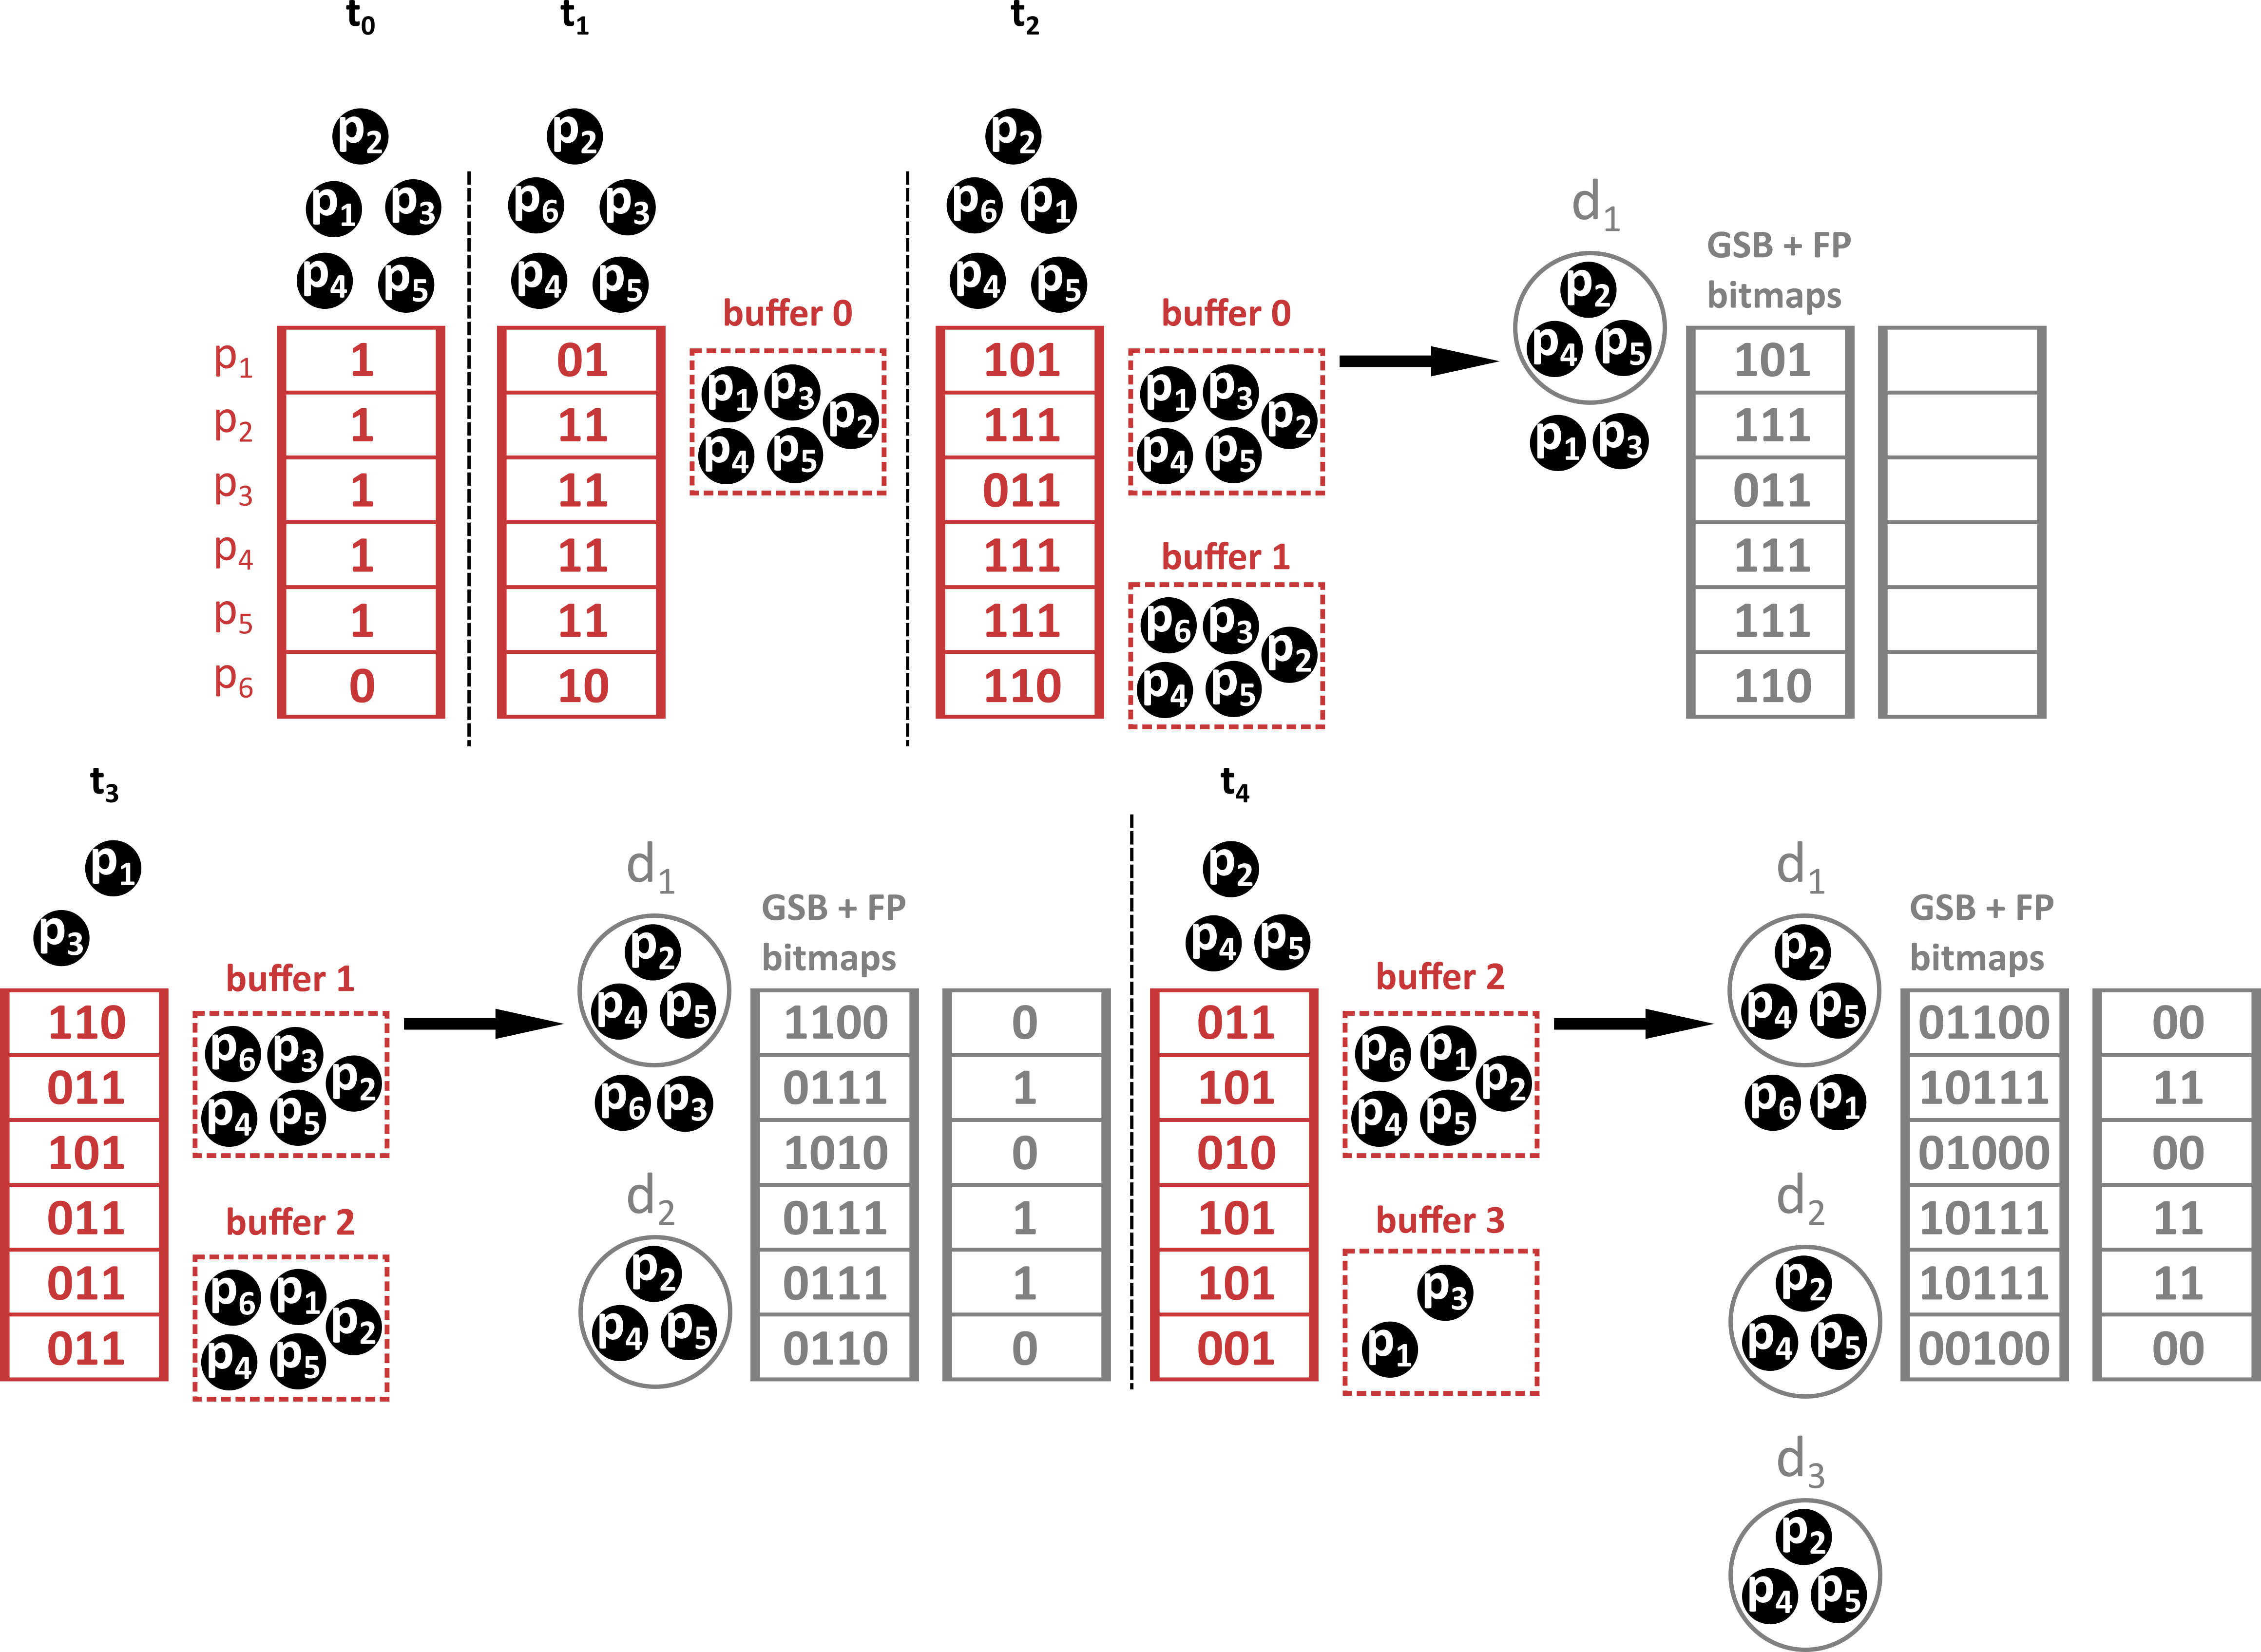
\includegraphics[width=\linewidth]{images/gsb_fp_flow.png}}
    \footnotesize{Source: Made by the author.}
    \label{fig:gsb_fp_flow}
\end{figure}

The same flow continues for time slot $t_3$, with \ac{gsb} sending the buffered points from time slot $t_1$ to \ac{fp}
for processing. We can now notice that the points that formed disk $d_1$ in the time slot $t_0$ now have a bit set to 1
in their presence bitmaps in \ac{fp}. Moreover, it is worth noting how we perform the bitmap concatenation in \ac{fp}
(when it receives points from $t_1$), in which the past time (\ac{fp} bitmaps) goes at the right and the future
(\ac{gsb} bitmaps) goes at the left side of the concatenated bitmap. We then perform a search for $\mu = 3$ bits set to
1 in that concatenated bitmaps to figure out which points can potentially form a flock pattern and can be placed in a
disk. Late in time slot $t_4$, when \ac{fp} receives the points from time slot $t_2$, a flock pattern will be found,
since we could find 3 consecutive disks containing at least $\mu = 3$ unique $O_{id}$.

\section{Taking Advantage of Multi-core Architectures}
\label{sec:multithread}
It's well known that multi-core architectures are the current trend in technology. There is a myriad of multi-core
processors in the market and many chipset companies taking advantages of those processor architectures too (even small
devices, like smartphones, are being shipped with multi-core processors). Given that current scenario, there is no sense
in not taking advantage of those multi-core processors and still executing our solution in a serial fashion. Thus, we
will remodel our proposed architecture in a multi-threaded structure and parallelize some of the expensive tasks that
our algorithm is doing, in order to make it more responsive and fast so it can empower decision makers to act in
real-time.

One can see that the \ac{fp} component, that we described in the previous section, is doing a lot of work in order to
discover the flock patterns. Whenever the \ac{fp} receives the set of points from \ac{gsb} it performs the following
actions:

\begin{enumerate}
    \item Build the whole point grid
    \item For each grid cell:
    \begin{enumerate}
        \item Get the \ac{egc} (e.g. for cell $c_{x,y}$ it will get cells $c_{x - 1, y - 1}...c_{x + 1, y+ 1}$)
        \item Process the \ac{egc}, trying to cluster the points into disks
    \end{enumerate}
    \item Get the resulting disks and assure that there are neither duplicates nor subsets of other disks
    \item Try to merge the disks with potential flocks from previous time slots
    \item Report new found flocks
\end{enumerate}

It can be easily perceived that the \ac{egc} processing (steps (a) and (b)) can be done in parallel for the multiple
cells that will be processed, since there is no dependency and no concurrent writing operations between cells. Another
step that is very \ac{cpu} heavy is the disk check described in step 3, but that step is very difficult to parallelize,
as we could see in Algorithm~\ref{alg:fp}. In that algorithm we showed that we start with an empty set of disks in the
beginning of the \textsc{Process} procedure and add disks to that set as we go finding them. However, before adding a
disk $d$ to the set, we check amongst the other disks that were previously there if $d$ is neither a subset nor a
superset of an existing disk. If $d$ is a subset, then it is not added to the set, but if $d$ is a superset of an
existing disk $d_2$, that disk $d_2$ is then removed from the set and $d$ is added instead (the superset check is done
inside the procedure \textsc{AddDisk}). Thus, if we try to parallelize that disk check procedure we would need to have
synchronizing primitives to protect the concurrent writing operations to the shared disk set, which could end up being
slower than executing it sequentially. Even without being able to fully parallelize the disk check steps, we can still
take advantage of other techniques to gain some speed in processing, like using the divide and conquer approach. The
idea would be to have multiple disk sets (one per independent worker thread processing \acp{egc}) and have each
independent thread add disks (and thus check for subsets/supersets) to its own set. When each worker thread has finished
its processing we would have each thread's set being merged with the global disk set in \ac{fp}, leaving less checks to
be performed by the global disk set.

\subsection{Multi-threaded Design}
\label{subsec:multithread}
The multi-threaded idea described in \secref{sec:multithread} can be modeled as a Producer-Multiple Consumers problem,
where we would have a single producer assembling the \ac{egc}s and multiple consumers taking a \ac{egc} from a shared
queue and clustering the points in the disks that it might find for that specific \ac{egc}. On a step further, each
consumer thread $c_t$ will also spawn another thread $d_t$ that will process disks that $c_t$ has found and will check
for subsets and supersets in its own private disk set.

\begin{figure}[h!]
    \centering
    \caption{Modeling the \ac{fp} in a Producer-Multiple Consumers architecture}
    \centerline{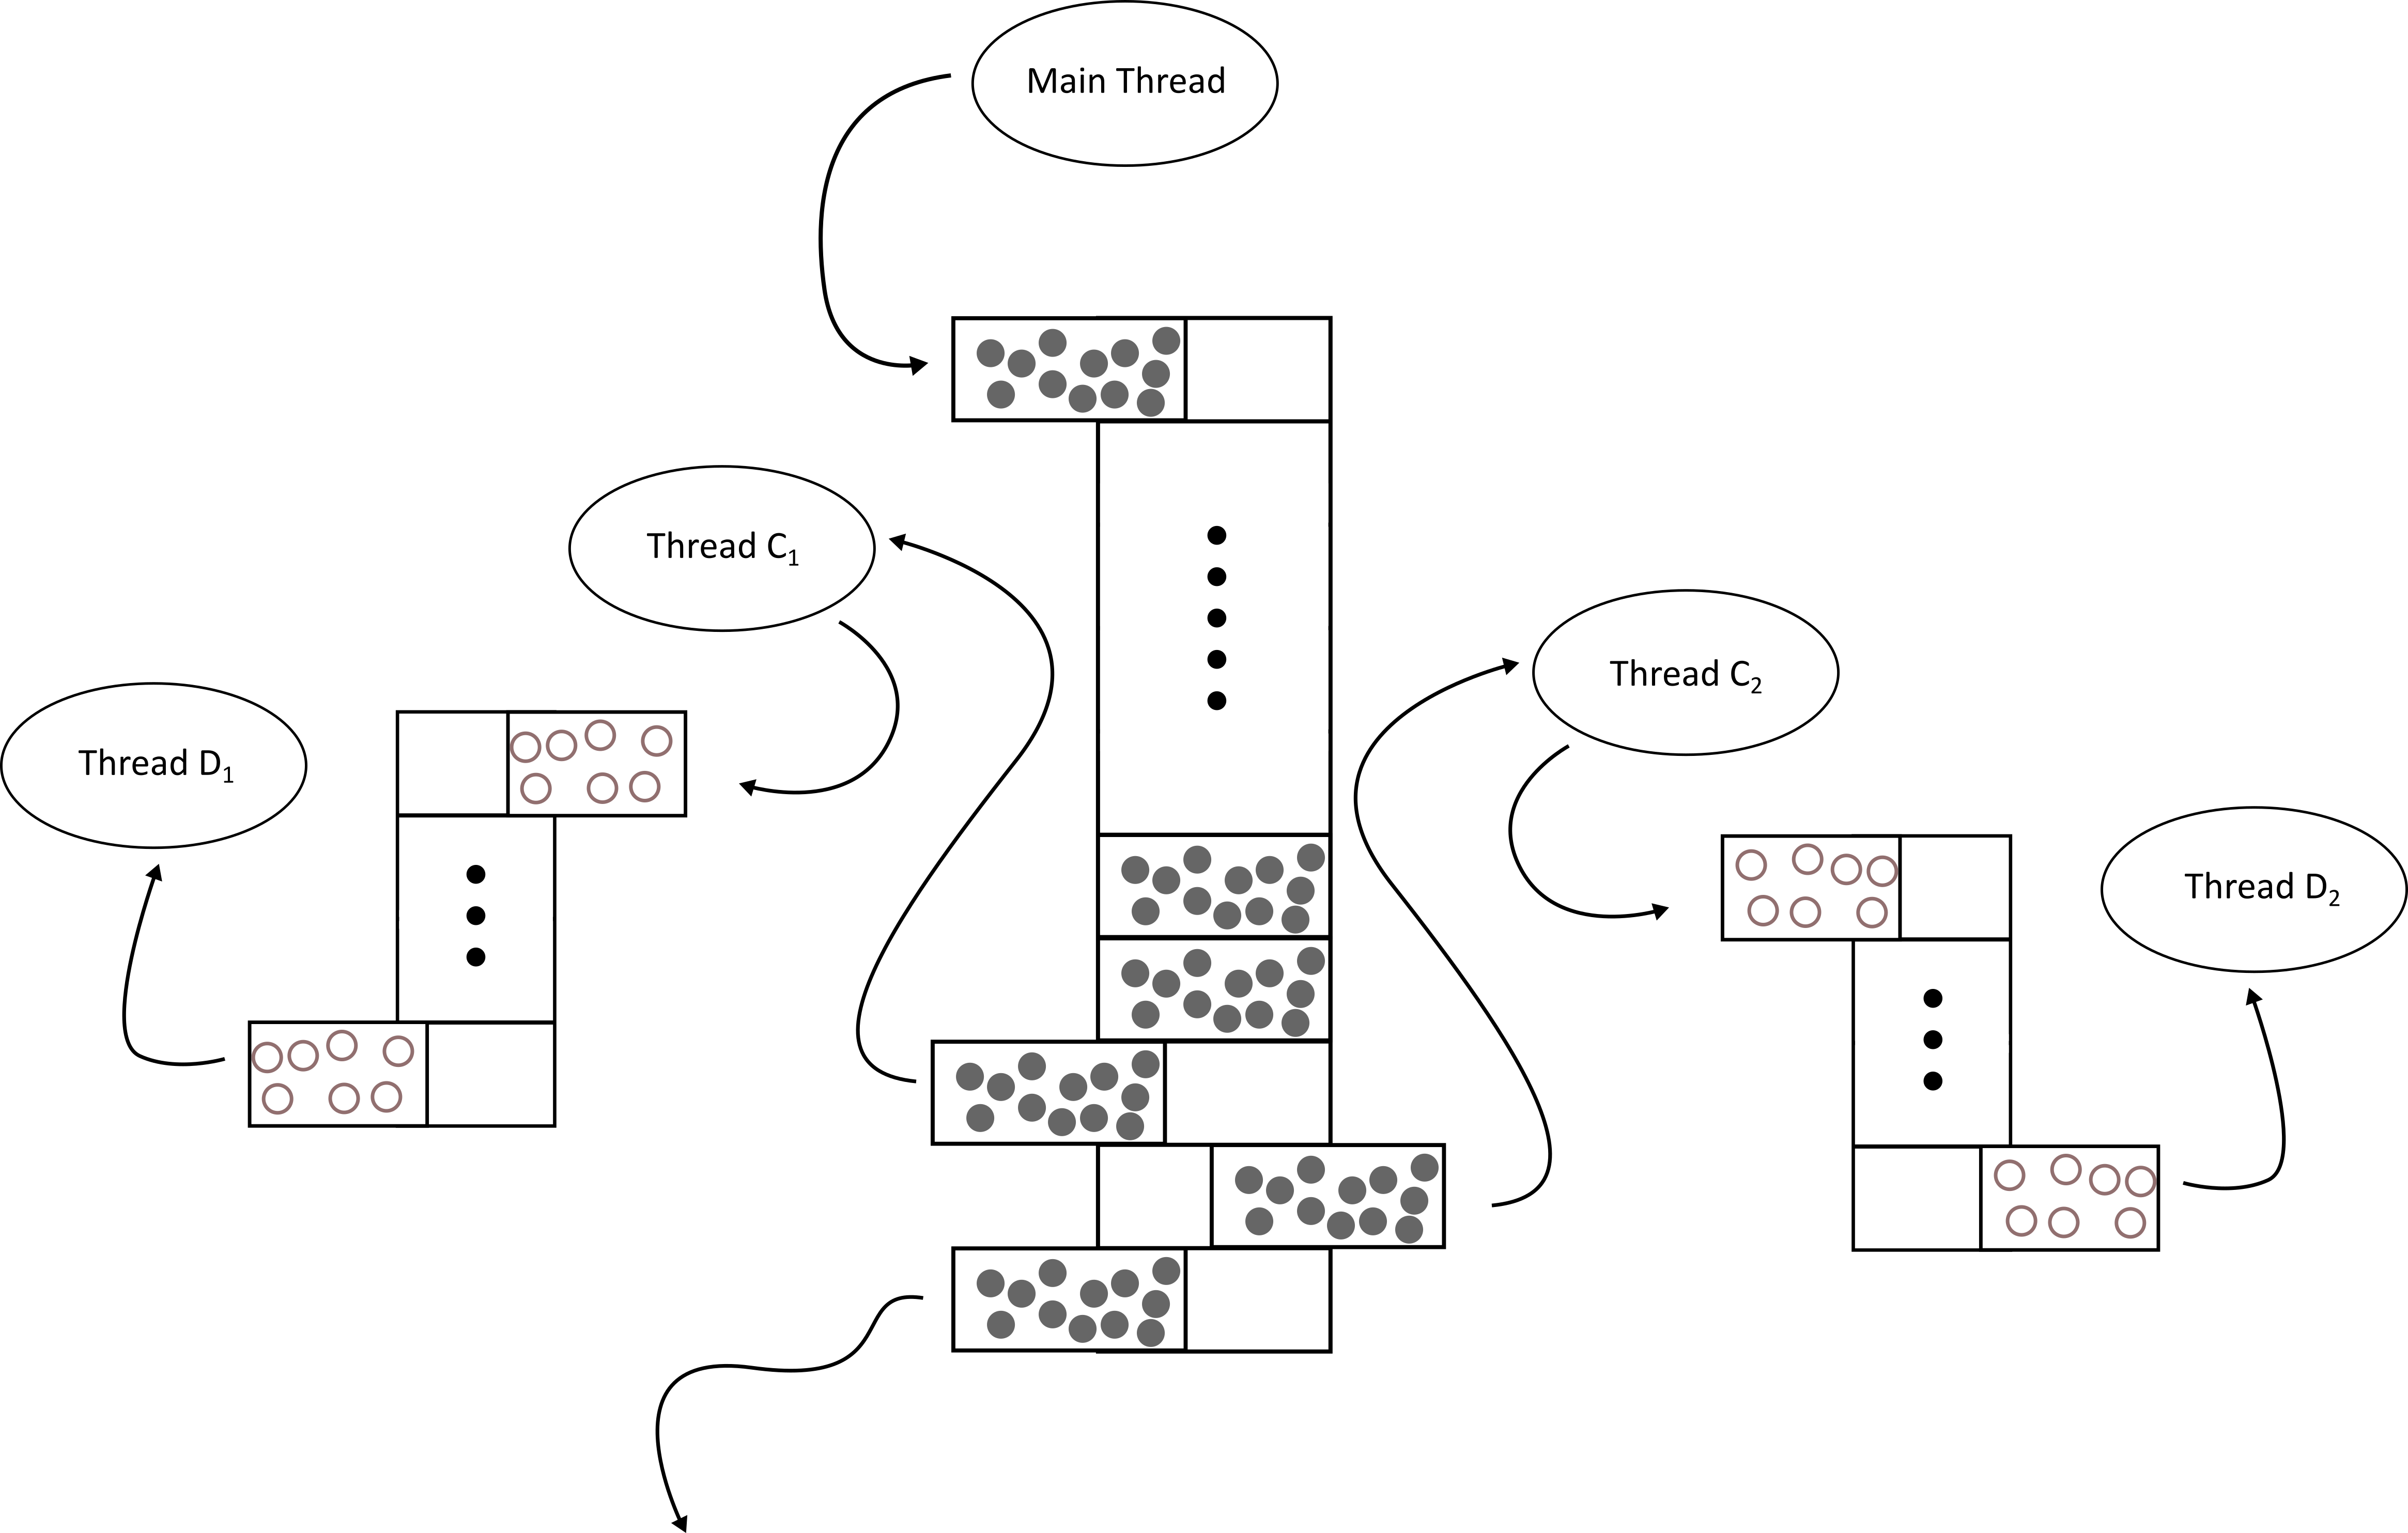
\includegraphics[width=\linewidth]{images/multithread.png}}
    \footnotesize{Source: Made by the author.}
    \label{fig:multithread}
\end{figure}

\figref{fig:multithread} illustrates how the \ac{fp} will be rearchitected in order to take advantage of parallel
execution.  We can see that the main thread will collect the \ac{egc} for each cell grid and enqueue it in a shared
queue that will be accessed by $N$ consumers. Whenever a consumer ($c_t$ thread) dequeues an \ac{egc}, it will then try
to find a pair of disks for each pair of points in the \ac{egc}, cluster the remaining points in those disks and then
enqueue those disks in another shared queue. Such shared queue will only be shared with the disk thread $d_t$ belonging
to the $c_t$ thread that created it. Then, each $d_t$ will be responsible to check for subsets and supersets in its own
set of disks, saving a lot of processing time when those disks are merged (and also checked for subsets and supersets)
with the global disk set in the \textsc{Process} procedure.
